% !TEX root = ../slides.tex
%%%%%%%%%%%%%%%%%%%%%%%%%%%%%%%%%%%%%%%%%%%%%%%%%%%%%%%%%%%%%%%%%%%%%%%%%%%%%%%%
% Session 9: Fourier series
%%%%%%%%%%%%%%%%%%%%%%%%%%%%%%%%%%%%%%%%%%%%%%%%%%%%%%%%%%%%%%%%%%%%%%%%%%%%%%%%

\session{session09}{Spectral methods}{Fourier series}
{Section 6.1}
{--}
{6.1}

\begin{frame}{Plan for today}
    \begin{enumerate}
        \item Continuous Fourier series and the truncation $P_N$.
        \item Periodic Sobolev spaces and the truncation error.
        \item Discrete Fourier series: interpolation $I_N$ and aliasing.
        \item Differentiation.
        \item Example: Fourier--Galerkin for the periodic Laplace equation.
    \end{enumerate}
    \bigskip
    \takeaway{Fourier series are the natural basis for periodic problems: derivatives become multiplications.}
\end{frame}

\begin{frame}{Continuous Fourier series}
    $\phi_k(x) = e^{ikx}$, $k \in \mathbb Z$, is an orthogonal system in $L^2(0,2\pi)$:
    \(
        \int_0^{2\pi} \phi_k \overline{\phi_l} = 2\pi\delta_{kl}.
    \)
    \begin{definition}[Fourier coefficients and truncation]
        \[
            \hat u_k = \frac{1}{2\pi} \int_0^{2\pi} u(x)\, \overline{\phi_k(x)} \diff x,
            \qquad
            Su = \sum_{k \in \mathbb Z} \hat u_k \phi_k,
            \qquad
            P_N u = \sum_{k = -N/2}^{N/2 - 1} \hat u_k \phi_k \quad (N \text{ even}).
        \]
        $S_N = \spannedby_{\mathbb C}\{\phi_k : -N/2 \le k \le N/2 - 1\}$.
    \end{definition}
    \begin{itemize}
        \item Parseval: $\|u\|^2_{L^2(0,2\pi)} = 2\pi \sum_k |\hat u_k|^2$. Hence $P_N u \to u$ in $L^2$ for every $u \in L^2(0,2\pi)$.
        \item If $u$ is periodic and $C^1$ (or Hölder), $P_N u \to u$ uniformly. Continuity alone is not enough.
        \item Real $u$: $\hat u_{-k} = \overline{\hat u_k}$, so $u = \sum a_k \cos kx + b_k \sin kx$ with $\hat u_k = a_k - i b_k$.
              For real approximations use symmetric frequencies $-K, \dots, K$ (i.e.\ $N = 2K+1$).
    \end{itemize}
\end{frame}

\begin{frame}{Gibbs' phenomenon}
    \begin{columns}[c]
        \begin{column}{.5\textwidth}
            \begin{example}
                \[
                    u(x) = \begin{cases} 1 & \frac\pi2 < x \le \frac{3\pi}{2}, \\ 0 & \text{otherwise}, \end{cases}
                \]
                \[
                    \hat u_k = \begin{cases}
                        \frac12                       & k = 0,              \\
                        0                             & k \ne 0 \text{ even}, \\
                        -\frac{(-1)^{(k-1)/2}}{k\pi}  & k \text{ odd}.
                    \end{cases}
                \]
            \end{example}
            \begin{itemize}
                \item Slow decay $|\hat u_k| \sim 1/k$: $u$ is discontinuous.
                \item Oscillations near the jumps that do not disappear as $N \to \infty$.
            \end{itemize}
        \end{column}
        \begin{column}{.48\textwidth}
            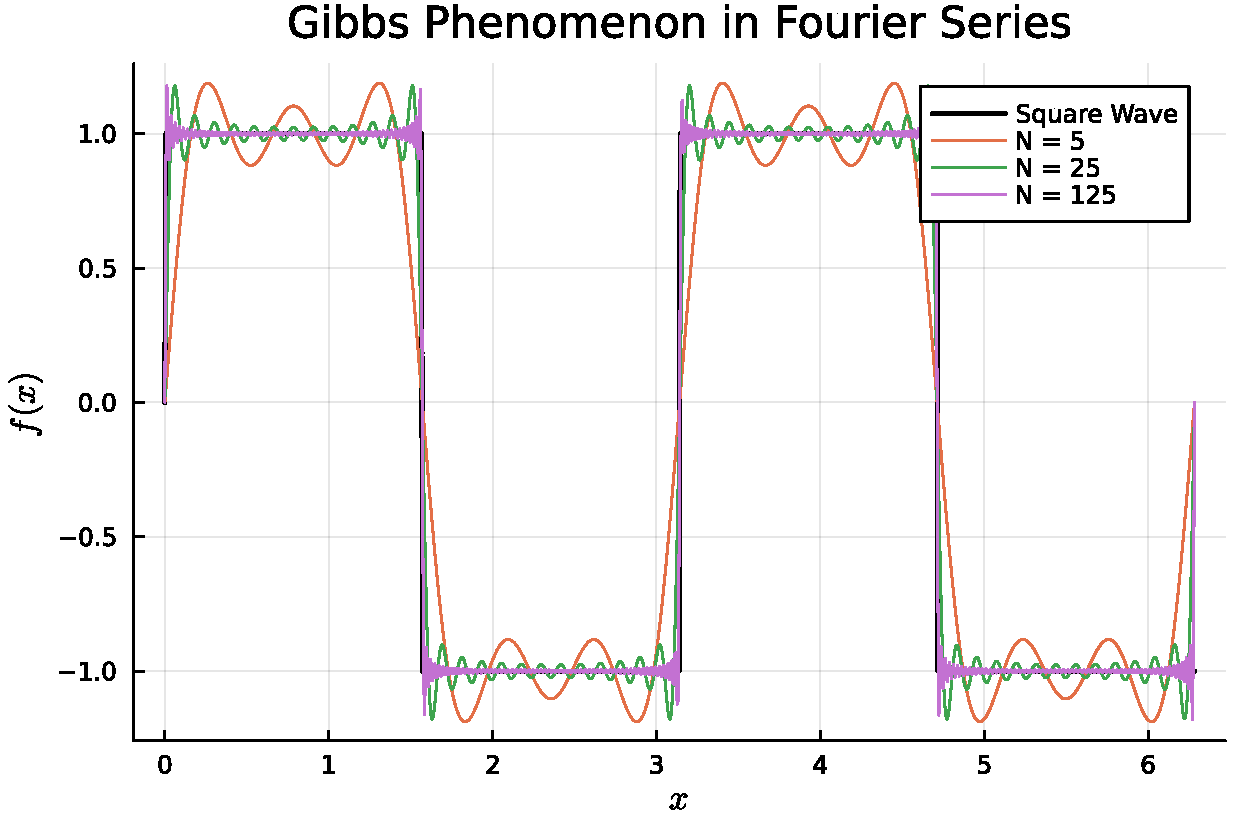
\includegraphics[width=\textwidth]{../../lectures/spectral/basis/Gibbs.pdf}
        \end{column}
    \end{columns}
    \takeaway{Smoothness of $u$ $\Longleftrightarrow$ fast decay of $\hat u_k$.}
\end{frame}

\begin{frame}{Periodic Sobolev spaces}
    \[
        C^m_p([a,b]) = \{ u \in C^m([a,b]) : u^{(k)}(a) = u^{(k)}(b),\ 0 \le k \le m \},
    \]
    \[
        H^m_p(a,b) = \text{closure of } C^m_p([a,b]) \text{ in } H^m(a,b).
    \]
    \begin{itemize}
        \item Derivatives in Fourier: $\widehat{(u')}_k = ik\, \hat u_k$ (for periodic $u$). \board{integrate by parts.}
        \item Equivalent norm in $H^m_p(0,2\pi)$:
              \[
                  \newnorm{u}_{H^m_p(0,2\pi)} = \Big( \sum_{k \in \mathbb Z} (1 + |k|^{2m}) |\hat u_k|^2 \Big)^{\frac 12}.
              \]
        \item $L^2_p = L^2$: $P_N u \to u$ in $L^2$ also for non-periodic $u$. But periodicity is needed for fast convergence.
    \end{itemize}
\end{frame}

\begin{frame}{Truncation error}
    \begin{theorem}[Truncation of the Fourier series of a periodic function]
        For integers $0 \le k \le m$ and $u \in H^m_p(0,2\pi)$,
        \[
            \|u - P_N u\|_{H^k(0,2\pi)} \le C N^{k-m} \|u^{(m)}\|_{L^2(0,2\pi)} .
        \]
    \end{theorem}
    \begin{proofsteps}[Proof for $k = 0$]
        By Parseval, and since $|k| \ge N/2$ for the omitted indices,
        \[
            \frac{1}{2\pi}\|u - P_N u\|^2_{L^2}
            = \sum_{k \notin [-\frac N2, \frac N2 - 1]} |\hat u_k|^2
            \le \Big(\frac N2\Big)^{-2m} \sum_{k \in \mathbb Z} |k|^{2m} |\hat u_k|^2
            = \frac{2^{2m}}{2\pi} N^{-2m} \|u^{(m)}\|^2_{L^2}.
        \]
    \end{proofsteps}
    \begin{itemize}
        \item Consequence: $\inf_{\phi \in S_N} \|u - \phi\|_{H^k} \le C N^{k-m} \|u^{(m)}\|_{L^2}$.
        \item If $u \in C^\infty_p$: faster than any power of $N$ (\alert{spectral accuracy}).
    \end{itemize}
\end{frame}

\begin{frame}{Discrete Fourier series}
    Nodes $x_j = \frac{2\pi j}{N}$, $j = 0, \dots, N-1$, and $u \in C_p([0,2\pi])$.
    \begin{definition}[Discrete Fourier coefficients]
        \[
            \tilde u_k = \frac 1N \sum_{j=0}^{N-1} u(x_j)\, \overline{\phi_k(x_j)}, \qquad k = -\tfrac N2, \dots, \tfrac N2 - 1.
        \]
    \end{definition}
    \begin{itemize}
        \item Discrete orthogonality: $\frac1N \sum_{j} \phi_l(x_j)\overline{\phi_k(x_j)} = 1$ if $l - k \in N\mathbb Z$, and $0$ otherwise.
        \item Hence $u(x_j) = \sum_k \tilde u_k \phi_k(x_j)$: the interpolant is
              \[
                  I_N u(x) = \sum_{k} \tilde u_k \phi_k(x) = \sum_{j=0}^{N-1} u(x_j)\, \psi_j(x),
                  \qquad
                  \psi_j(x) = \frac1N \sum_{k=-N/2}^{N/2-1} \phi_k(x - x_j),
              \]
              with $\psi_j(x_l) = \delta_{jl}$.
        \item The $\tilde u_k$ are computed with the Fast Fourier Transform in $O(N\log N)$ operations.
    \end{itemize}
\end{frame}

\begin{frame}{Aliasing}
    On the grid, high frequencies look like low ones: \ $e^{i(k + Nl)x_j} = e^{ikx_j}$ for $l \in \mathbb Z$.
    \medskip

    For $u \in H^m_p(0,2\pi)$ with $m \ge 1$:
    \[
        \tilde u_k = \sum_{l \in \mathbb Z} \hat u_{k + Nl}
        \qquad \Longrightarrow \qquad
        I_N u = P_N u + R_N u, \qquad
        R_N u = \sum_{k = -N/2}^{N/2-1} \Big( \sum_{l \ne 0} \hat u_{k+Nl} \Big) \phi_k .
    \]
    \begin{itemize}
        \item $R_N u$ is the \alert{aliasing error}. By orthogonality,
              \[
                  \|u - I_N u\|^2_{L^2} = \|u - P_N u\|^2_{L^2} + \|R_N u\|^2_{L^2}.
              \]
        \item It is of the same order as the truncation error:
              \[
                  \|R_N u\|_{L^2} \le C N^{-m} \|u^{(m)}\|_{L^2(0,2\pi)} .
              \]
    \end{itemize}
    \takeaway{Interpolation is (almost) as good as projection, and much cheaper.}
\end{frame}

\begin{frame}{Differentiation}
    \begin{definition}[Fourier interpolation derivative]
        \[
            \mathcal D_N u \defeq \frac{\diff}{\diff x} (I_N u) = \sum_{k} ik\, \tilde u_k \phi_k .
        \]
    \end{definition}
    \begin{itemize}
        \item In general $\mathcal D_N u \ne P_N u'$ and $\mathcal D_N u \ne I_N u'$.
        \item In practice: values $\xrightarrow{\text{FFT}}$ $\tilde u_k$ $\xrightarrow{\times ik}$ $ik\tilde u_k$ $\xrightarrow{\text{inverse FFT}}$ values of $\mathcal D_N u$.
        \item Equivalently, a differentiation matrix $\mat D_N$ acting on the nodal values (Session 8).
    \end{itemize}
\end{frame}

\begin{frame}{Example: periodic Laplace equation by Fourier--Galerkin}
    \[
        -u'' = f \text{ in } (0,2\pi), \qquad u(0) = u(2\pi),\ u'(0) = u'(2\pi), \qquad f \text{ real}.
    \]
    \begin{itemize}
        \item Compatibility: $\int_0^{2\pi} f = 0$, i.e.\ $\hat f_0 = 0$. Solutions are unique up to constants: impose $\int_0^{2\pi} u = 0$.
        \item $V = \{u \in H^1_p(0,2\pi;\R) : \int_0^{2\pi} u = 0\}$, \ $\int_0^{2\pi} u'\phi' = \int_0^{2\pi} f \phi$ for all $\phi \in V$.
        \item Testing with $\cos kx$, $\sin kx$: \quad $k^2 \hat u_k = \hat f_k$, $k \ne 0$, so
              \[
                  u = \sum_{k \ne 0} \frac{\hat f_k}{k^2} \phi_k .
              \]
        \item Galerkin with $N = 2K+1$ real modes, $V_N = V \cap \spannedby_\R\{1, \cos x, \sin x, \dots, \cos Kx, \sin Kx\}$:
              \[
                  u_N = \sum_{0 < |k| \le K} \frac{\hat f_k}{k^2} \phi_k = Q_N u \quad \text{(the truncation of } u\text{)}.
              \]
    \end{itemize}
\end{frame}

\begin{frame}{The example in terms of Céa and Aubin--Nitsche}
    $a(u,v) = \int_0^{2\pi} u'v'$ is continuous, symmetric and coercive on $V$ (Poincaré--Wirtinger). Let $h = N^{-1}$.
    \begin{itemize}
        \item Céa $+$ truncation error with $u \in H^{m+2}_p$ (if $f \in H^m_p$):
              \[
                  \|u - u_N\|_{H^1(0,2\pi)} \le C \|u - Q_N u\|_{H^1(0,2\pi)} \le C h^{m+1} \|f^{(m)}\|_{L^2(0,2\pi)} .
              \]
        \item Aubin--Nitsche with $H = L^2_0$ and $\omega(h) = Ch$:
              \[
                  \|u - u_N\|_{L^2(0,2\pi)} \le C h^2 \|f\|_{L^2(0,2\pi)} .
              \]
    \end{itemize}
    \takeaway{The order of convergence is limited only by the smoothness of $f$.}
\end{frame}

\begin{frame}{Summary and practice}
    \begin{itemize}
        \item $P_N u$: truncated Fourier series; error $O(N^{k-m})$ in $H^k$ for $u \in H^m_p$.
        \item $I_N u$: interpolation at $x_j = 2\pi j/N$; error $=$ truncation $+$ aliasing, same order.
        \item Derivatives: multiplication by $ik$ (FFT).
        \item Fourier--Galerkin for the periodic Laplacian: $u_N = Q_N u$.
    \end{itemize}
    \bigskip
    \textbf{Practice.} Exercise 6.1:
    \begin{itemize}
        \item Code the Fourier--Galerkin method for the periodic Laplacian (use a library for the integrals $\hat f_k$).
        \item Code the Fourier collocation method with $N = 2K+1$ nodes. Solvability requires $\sum_j f(x_j) = 0$: subtract the mean of the samples if necessary.
        \item Compare the errors as functions of $N$.
    \end{itemize}
    \bigskip
    \textbf{Next session:} orthogonal polynomials (non-periodic problems).
\end{frame}
